\chapter{Results}\label{ch:results}\addtocontents{lof}{\protect\contentsline{chapter}{\protect\numberline{\thechapter}Results}{}{}}
% \newthought{Synopsis}\synopsisMethod
The results of the testing of the proof of concept rig are presented in this chapter. The results are presented in a qualitative manner as the rig was not designed to provide quantitative results.
The goal of the testing was to determine if the proof of concept rig was able to simulate the coaptation of the tricuspid valve and the flow of blood through the valve, if the valve leaflets and chordae tendineae could sustain the systolic pressure developed from coaptation, verifying the functionality of the valve for use in the right-heart simulator and later integration of CroiValve DUO.
\section{Design evaluation and thickness investigaton}
Differences in cast parts with and without tendineae\todo{flesh out section, populate table}
(Table of thickness results)

\section{Pilot Tests}
The teflon tape worked very well where applied however the 3D-printed end cap of the core testing chamber leaked a lot even after an attempt to seal with tack. This was due to a mis-fitting of the O-ring used on the part.

\section{Coaptation Test}
The valve part coapted well, septal and posterior leaflets in particular, the cusp of the anterior leaflet however didnt coapt with either of the adjacent two creating a larger regurgitant orifice than expected. This is likely due to;
\begin{itemize}
    \item The material properties of the \gls{PU} used not being elastic enough.
    \item The thickness of the leaflets being too thick making them less flexible.
    \item The overlapping length of nylon wire on the leaflets making them stiffer.
    \item The natural saddle shape of the valve annulus being flattened off to fit in the seating fixture.
    \item Leaflets length loss from the processing of the valve model.
\end{itemize}

The chordae tendineae held up well under the pressure and prevented the valve from prolapsing. They were tensioned to a point where they valve were allowed to partially prolapse similar to how native \gls{TV}'s do in regurgitant cases and an expected degree of prolapse occured as a result.

During assembly one of the chordae on the posterior leaflet broke leaving just two although this didn't majorly effect test results.

\begin{figure}
    \begin{fullwidth}
        \centering
        \subfloat[Head-On View]{%
            \href{https://drive.google.com/file/d/1epMX5xH8P03QeNA2DaLtc610iFQK58KK/view?usp=sharing}{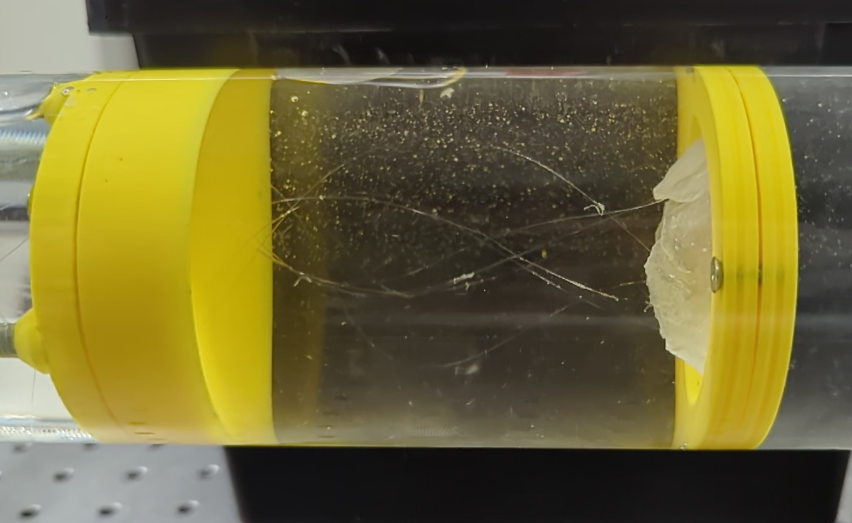
\includegraphics[width=0.45\linewidth]{figures/valverigcloseup}}%
        }\quad
        \subfloat[Oblique View]{%
            \href{https://drive.google.com/file/d/1RXlcIPh9iO5SNXvG8wYL6XBqwaXyd4fS/view?usp=sharing}{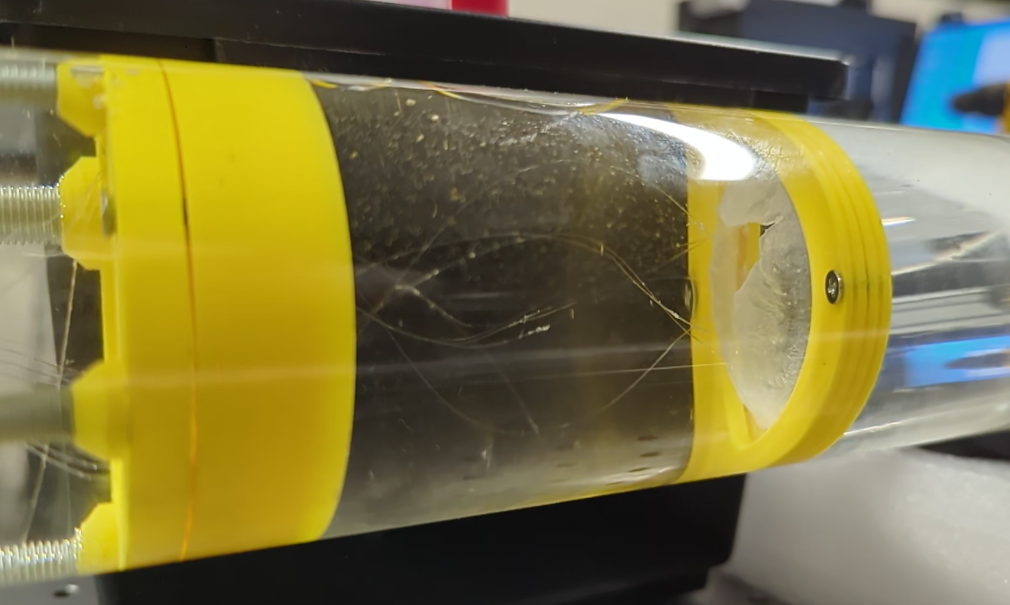
\includegraphics[width=0.45\linewidth]{figures/valverigcloseup2}}
        }
        \caption{Frame from video of valve coapting during testing \textbf{(click to view video)}}
        \label{fig:Videos}
    \end{fullwidth}
\end{figure}